%%%%%%%%%%%%%%%%%%%%%%%%%%%%%%%%%%%%%%%%%%%%%
\section{Study of the systematic uncertainties}
\label{sec:systematics}
%%%%%%%%%%%%%%%%%%%%%%%%%%%%%%%%%%%%%%%%%%%%%
%We estimate the systematic uncertainty on the post-corrections muon momentum 
%as the linear sum of two contributions accounting for the two common use cases:
The validation procedure described in the previous section is used for
estimating the systematic error on the post-correction momentum of the muons.

There are two common use cases for defining a systematic
error on the momentum scale: 
\begin{itemize}
\item {\sl Case I}: analyses where the spectrum in the data is compared
  with a model known from the simulation. Here the systematic error is
  indicated by the residual
  discrepancy between the post-correction
  spectrum in the data and in the simulation.
\item {\sl Case II}: analyses aiming to perform an absolute measurement of the
  momentum of the muon, e.g. not relying on a model for the
  expected spectrum. In this case, values of observables built from the measured
  momenta, namely invariant masses, differing from standard
  references are indications of systematic errors. 
\end{itemize}

\underline{\sl Case I}: We define the systematic error  $\Delta p_T$ related to the remaining discrepancy between
the data and the simulation as:
\begin{equation}
  \frac{\Delta p_T}{p_T}=\frac{M_{DATA}-M_{MC}}{M_{PDG}}
  \label{eq:syst_DATA_MC}
\end{equation}
The above relation between momentum
and masses holds under the hypothesis that the systematic errors are fully correlated between the two muons. 
The fractional difference on the mass is shown as a function of $|\eta|$ or $p_T$ of one of the two muons in
Figure~\ref{fig:ScaleDATAMC_8TeV}.
%%~\ref{fig:syst_DATA_MC_eta}. 
%% \begin{figure}[hbtp]  
%% \begin{center}
%% 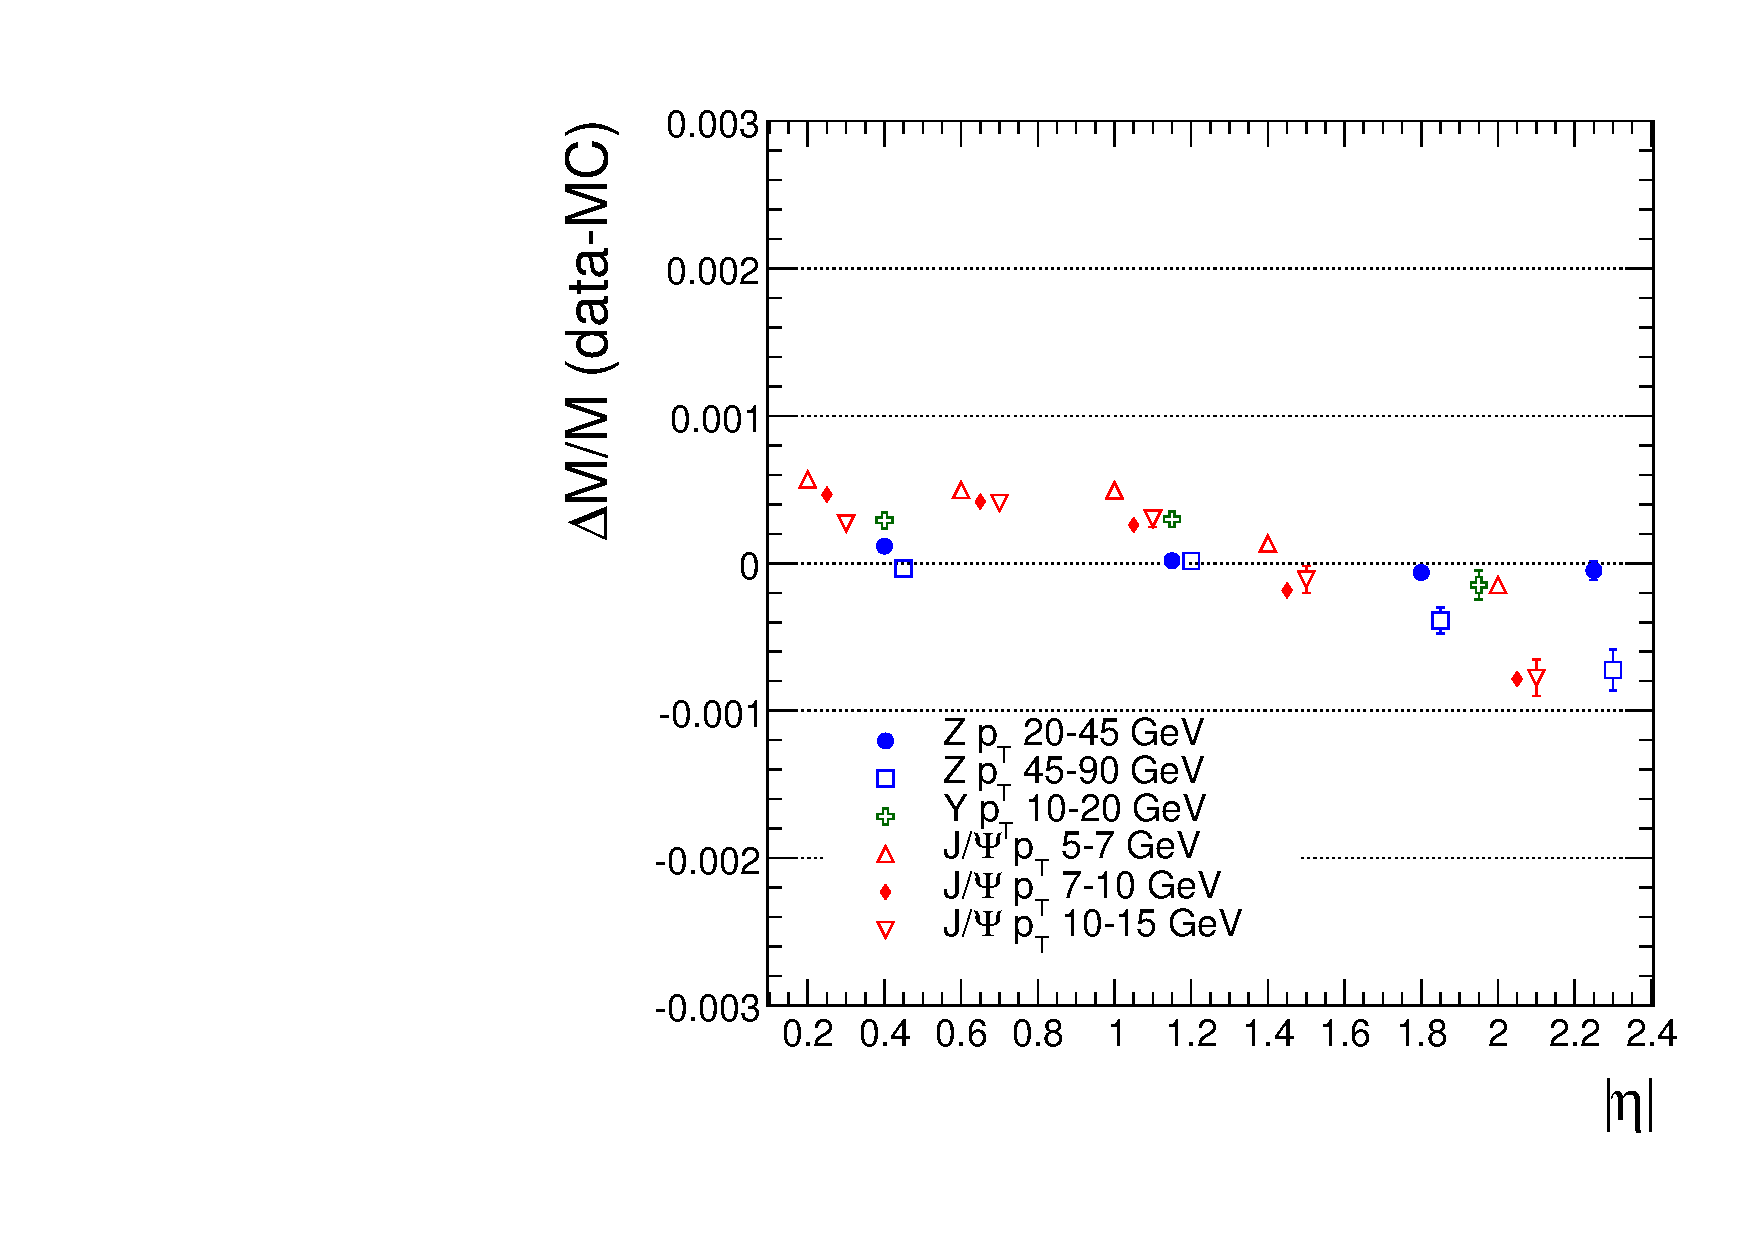
\includegraphics[width=\textwidth]{figures/ScaleEta_afterCorrection_V2}
%%  \hspace{1cm} 
%%    \caption{Fractional difference $\frac{M_{DATA}-M_{MC}}{M_{DATA}}$
%%      for dimuons from J/$\psi$, $\Upsilon(1S)$ and Z decays as a function of the $|\eta|$
%%      of one the two muons (averaged on the second).} 
%%    \label{fig:syst_DATA_MC_eta} 
%%  \end{center}
%% \end{figure} 
The fractional difference is everywhere well within $\pm$0.10\% with the largest value
being around -0.10\%, for the point in the large $|\eta|$ and $p_T$ bin.
Conservatively we assign a $\pm$0.05\% uncertainty everywhere apart from this
point where a $\pm$0.10\% uncertainty is assumed. 

\underline{\sl Case II}: With respect the previuos case, the
systematic error on $p_T$ has an additional contribution that we
evaluate using the simulation and taking as estimator the discrepancy
between the values of the mass of the Z boson extracted from the
spectra of the dimuons and the world average reported by the Particle
Data Group (PDG)~\cite{Beringer:1900zz}: 
\begin{equation}
  \frac{\Delta p_T}{p_T}=\frac{M_{MC}-M_{PDG}}{M_{PDG}}
  \label{eq:syst_MC_PDG}
\end{equation}
The above relation between momentum
and masses holds under the hypothesis that the systematic errors are fully correlated between the two muons. 
%Ideally after the calibration procedure, both in
%the simulation and in the data, 
We checked the behaviour of the fractional mass difference defined
in Eq.~\ref{eq:syst_MC_PDG} against $p_T$ and $|\eta|$ of one of the two
muons using simulated events reconstructed in realistic conditions
(Figure~\ref{fig:ScalePDGMC_8TeV}). 
%%%%
\begin{figure}[hbtp]  
\begin{center}
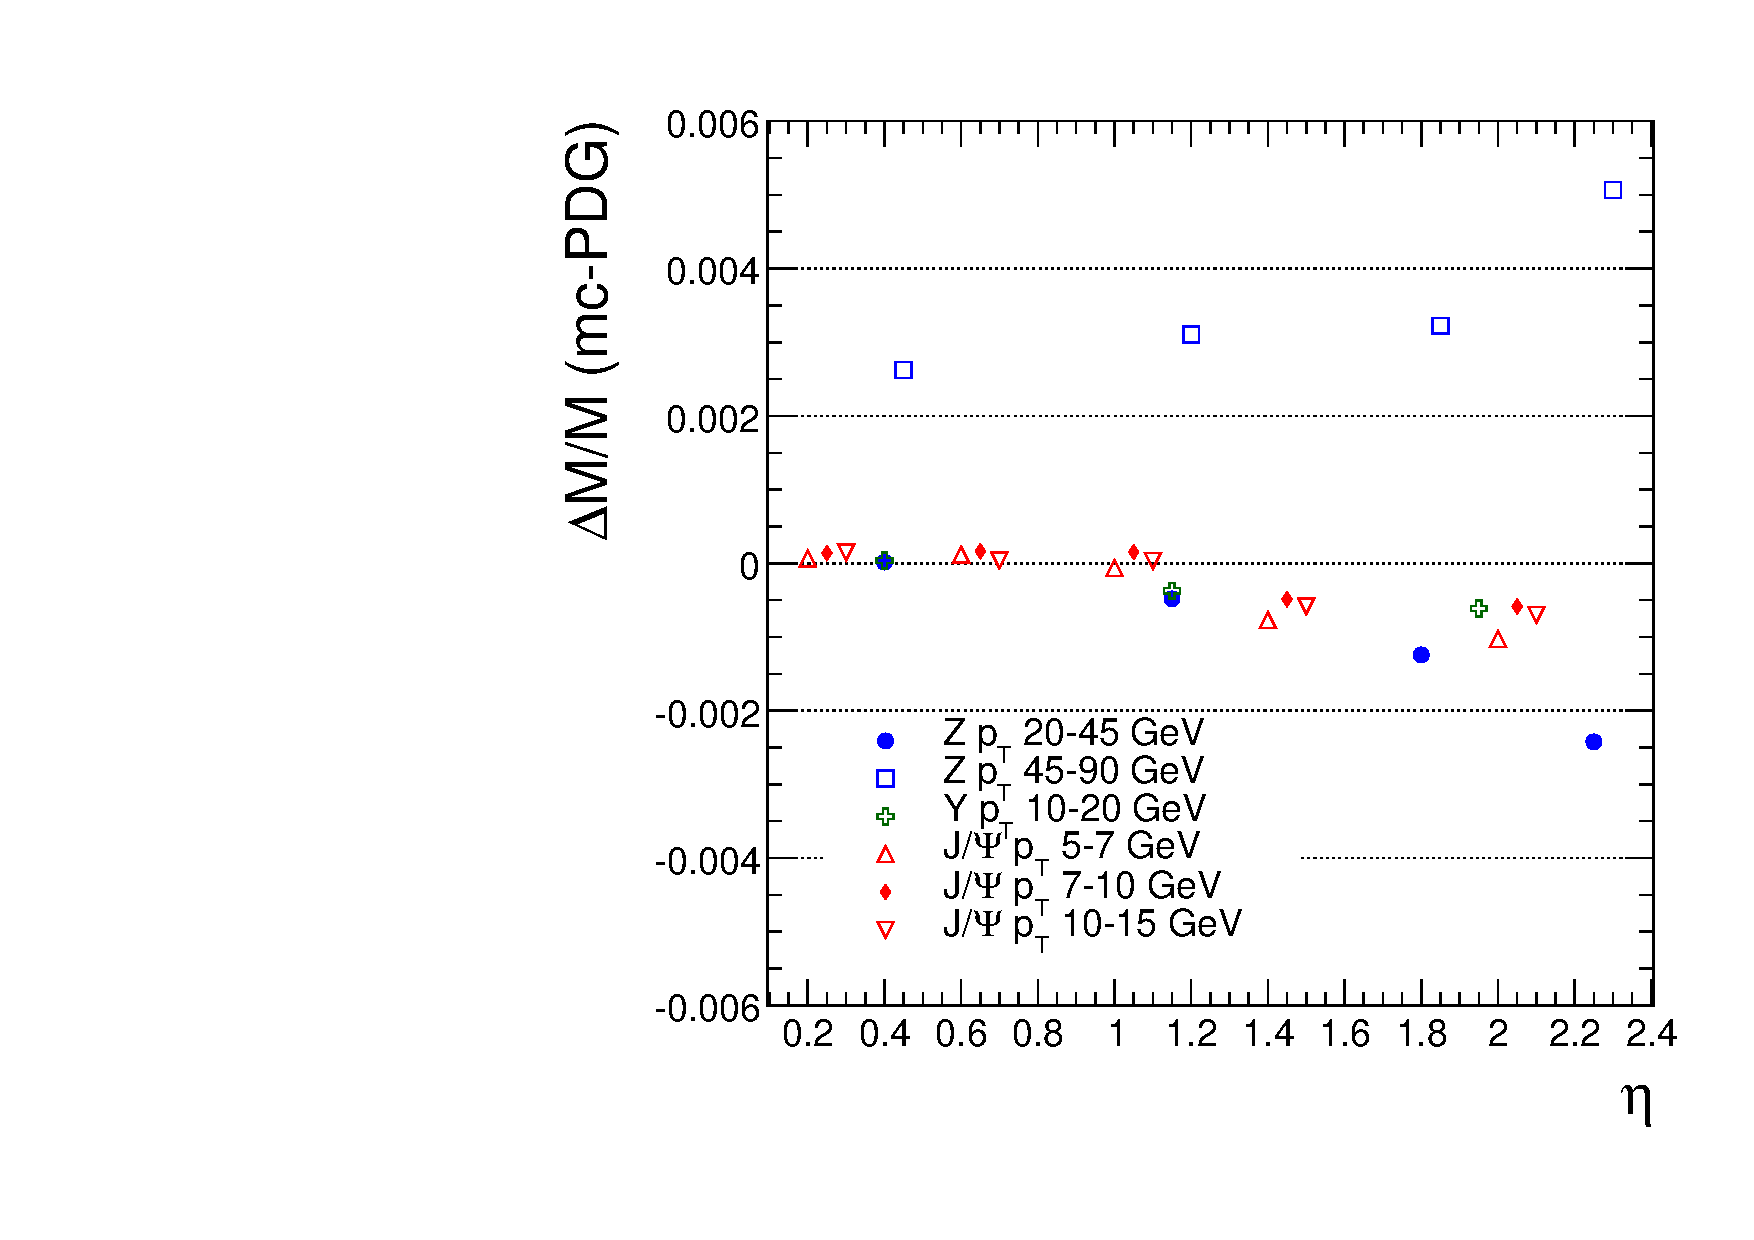
\includegraphics[width=0.7\textwidth]{figures/H4l_Style/2012_22Jan2013ReReco/ScalePdg_mc_Eta_afterCorrection_V2}
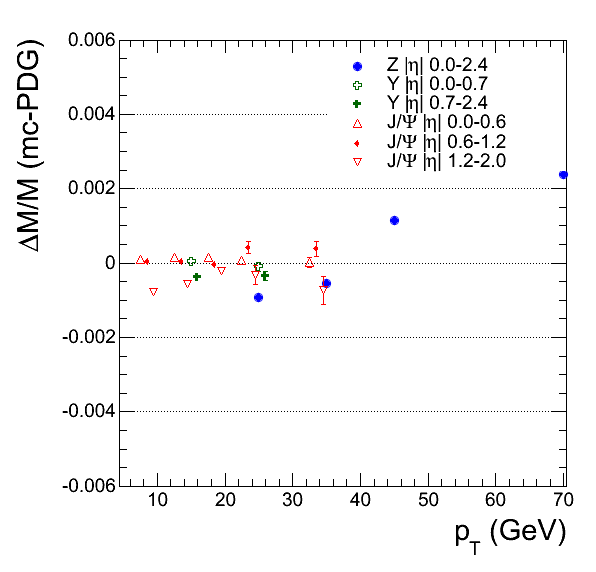
\includegraphics[width=0.7\textwidth]{figures/H4l_Style/2012_22Jan2013ReReco/ScalePdg_mc_Pt_afterCorrection_V2} 
 \hspace{1cm} 
   \caption{Fractional difference, PDG with respect simulation, of the fitted mass for the J/$\psi$,
     $\Upsilon(1S)$ and Z resonances as a function of the $|\eta|$ (top)
     and $p_T$ (bottom) of one of the two muons. Bars are the
     statistical error on the mass of the resonance from the fit.
   \label{fig:ScalePDGMC_8TeV}}
 \end{center}
\end{figure} 
Discrepancies from the PDG values, especially visible in the case of
the dimuons from Z, arise either
from a poor parametrization of the dimuon spectrum used to extract $M_{MC}$ or from biases on the muon momentum not entirely corrected by the
calibration procedure.
% %%%
% realistic conditions -> 
% which should reflect the
% level of knowledge of the calibration and alignment conditions which
% reflects their accuracy in the data. 
% %%%  TO BE DEFINED IN EARLIER  SECTIONS 
Since a not null value contributes 
to the {\sl Case II} error,
we disentangled the two effects using
simulated events reconstructed using the so-called {\sl ideal}
conditions , e.g. assuming a perfect knowledge of the
calibration and alignment conditions but with the same set of
dead channels as in real data.
In this sample, biases in the measured momentum due
to approximations in the track reconstruction (e.g. mismodelling
of the interaction of the charged particle
with the material or with the magnetic field during the reconstruction step) were the same as
in the reference sample reconstructed with realistic conditions. 
No MuScleFit corrections were applied to the muons reconstructed with ideal conditions.
Details on the samples used for this test are given in Table~\ref{tab:datasets_for_systematics}.
%%%%%%%
\begin{table}[hbH]
\begin{center}
\caption{Datasets \label{tab:datasets_for_systematics}} 
\begin{tabular}{|l|c|c|c|c|}
\hline
Dataset & MC generator & Data-Tier & events & Corrections applied\\
\hline 
DYJetsToLL & MadGraph &  AODSIM              & 2.95 M & MuScleFit \\
DYToMuMu   & POWHEG   &  AODSIM              & 8.60 M & MuScleFit \\
DYToMuMu   & POWHEG   &  START\_53 from RECO & 0.59 M & MuScleFit \\
DYToMuMu   & POWHEG   &  MC\_53 from RECO    & 0.59 M & nocorrections \\
\hline
\hline
\end{tabular}
\end{center}
\end{table}
%%%%
\begin{figure}[hbtp]  
\begin{center}
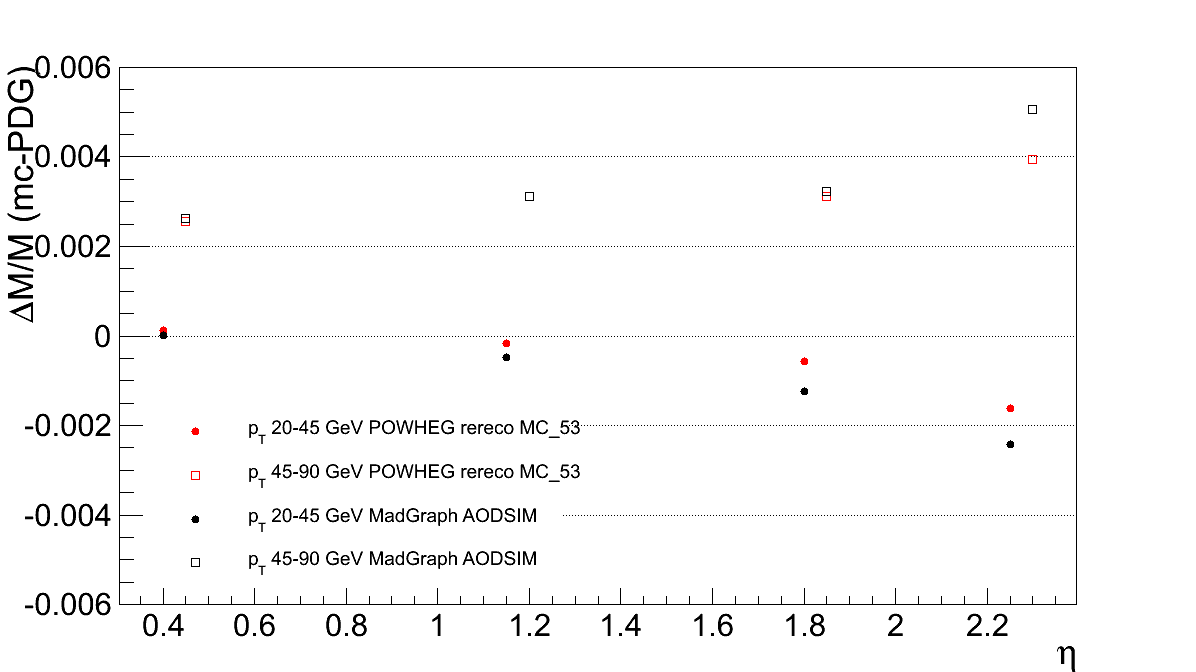
\includegraphics[width=\textwidth]{figures/ScalePdg_mc_Eta_Z}
 \hspace{1cm} 
   \caption{Fractional difference, PDG with respect simulation,
     for dimuons from Z bosons decays as a function of the $|\eta|$
   of one the two muons (averaged on the second).} 
   \label{fig:syst_MC_PDG_eta} 
 \end{center}
\end{figure} 
%Figure~\ref{fig:syst_MC_PDG_pT} shows the fractional difference on the
%mass as a function of $p_T$ of one of the
%two muons. Points for realistic simulation (post-correction) show a
%bias increasing with $p_T$. The same trend is observed for the points
%obtained with the ideal simulation which agree the with the others 
%at the 0.0005 level on all the $p_T$ range. 

Figure~\ref{fig:syst_MC_PDG_eta} shows the fractional difference on
the mass as a function of $|\eta|$ of one of the two muons in two
different ranges of $p_T$ for the ideal and the realistic samples:
\begin{itemize}
\item for $p_T$ in the range [20,45] GeV, values
form the realistic simulation (post-correction) are off of about -0.05\%
for $|\eta|<$1.5 increasing up to -0.20\% at the largest $|\eta|$.
A similar trend, but with smaller offsets, is observed for points from the simulation in ideal
conditions. 
\item for $p_T$ in the range [45,90] GeV there is approximately
a +0.20\% bias growing up to +0.50\% at the largest $|\eta|$ bin
in case of both ideal and realistic conditions. 
\end{itemize}
For the muons in the sample reconstructed with ideal conditions, 
we found that the bias in the mass was similar to what determined
comparing the reconstructed $p_T$ with the value from the
MC-truth. This test indicates the overall reliablility of the fits
to the dimuon spectra. Consequently we used the fractional differences
defined by Eq.~\ref{eq:syst_MC_PDG} to estimate the difference between 
true and reconstructed $p_T$ in the realistic simulation.

Based on this analysis, the systematic errors on the momentum scale of
muons in the data, estimated for the
different $p_T$ and $|\eta|$ ranges are those summarized in
Table~\ref{tab:systematics}. {\sl Case II} systematic errors are the sum of the
second and third columns in the table.
%%%%%%%
\begin{table}[hbH]
\begin{center}
\caption{Estimated systematic uncertainties on the momentum scale
  of muons, post-correction, reconstructed in the data ($\Delta p_T/p_T$).
  Second column corresponds to {\sl Case I} systematics, while
  the sum of second and third columns corresponds to {\sl Case II}
  systematics described in the text.\label{tab:systematics}} 
\begin{tabular}{|l|c|c|}
\hline
 & DATA - MC & MC - PDG \\
\hline 
$p_T<$45 GeV,   0$<|\eta|<$1.5 & $\pm$0.05\%& $\pm$0.05\% \\
$p_T<$45 GeV, 1.5$<|\eta|<$2.4 & $\pm$0.10\%& $\pm$0.20\% \\
$p_T>$45 GeV,   0$<|\eta|<$2.0 & $\pm$0.05\%& $\pm$0.30\% \\
$p_T>$45 GeV, 2.0$<|\eta|<$2.4 & $\pm$0.10\%& $\pm$0.50\% \\
\hline
\hline
\end{tabular}
\end{center}
\end{table}
%%%%
